% =============================================
% 导言区
% =============================================
\documentclass{xjtureport}








% =============================================
% 正文区
% =============================================


\begin{document}

% ===导入实验报告封面==============================
\begin{titlepage}
	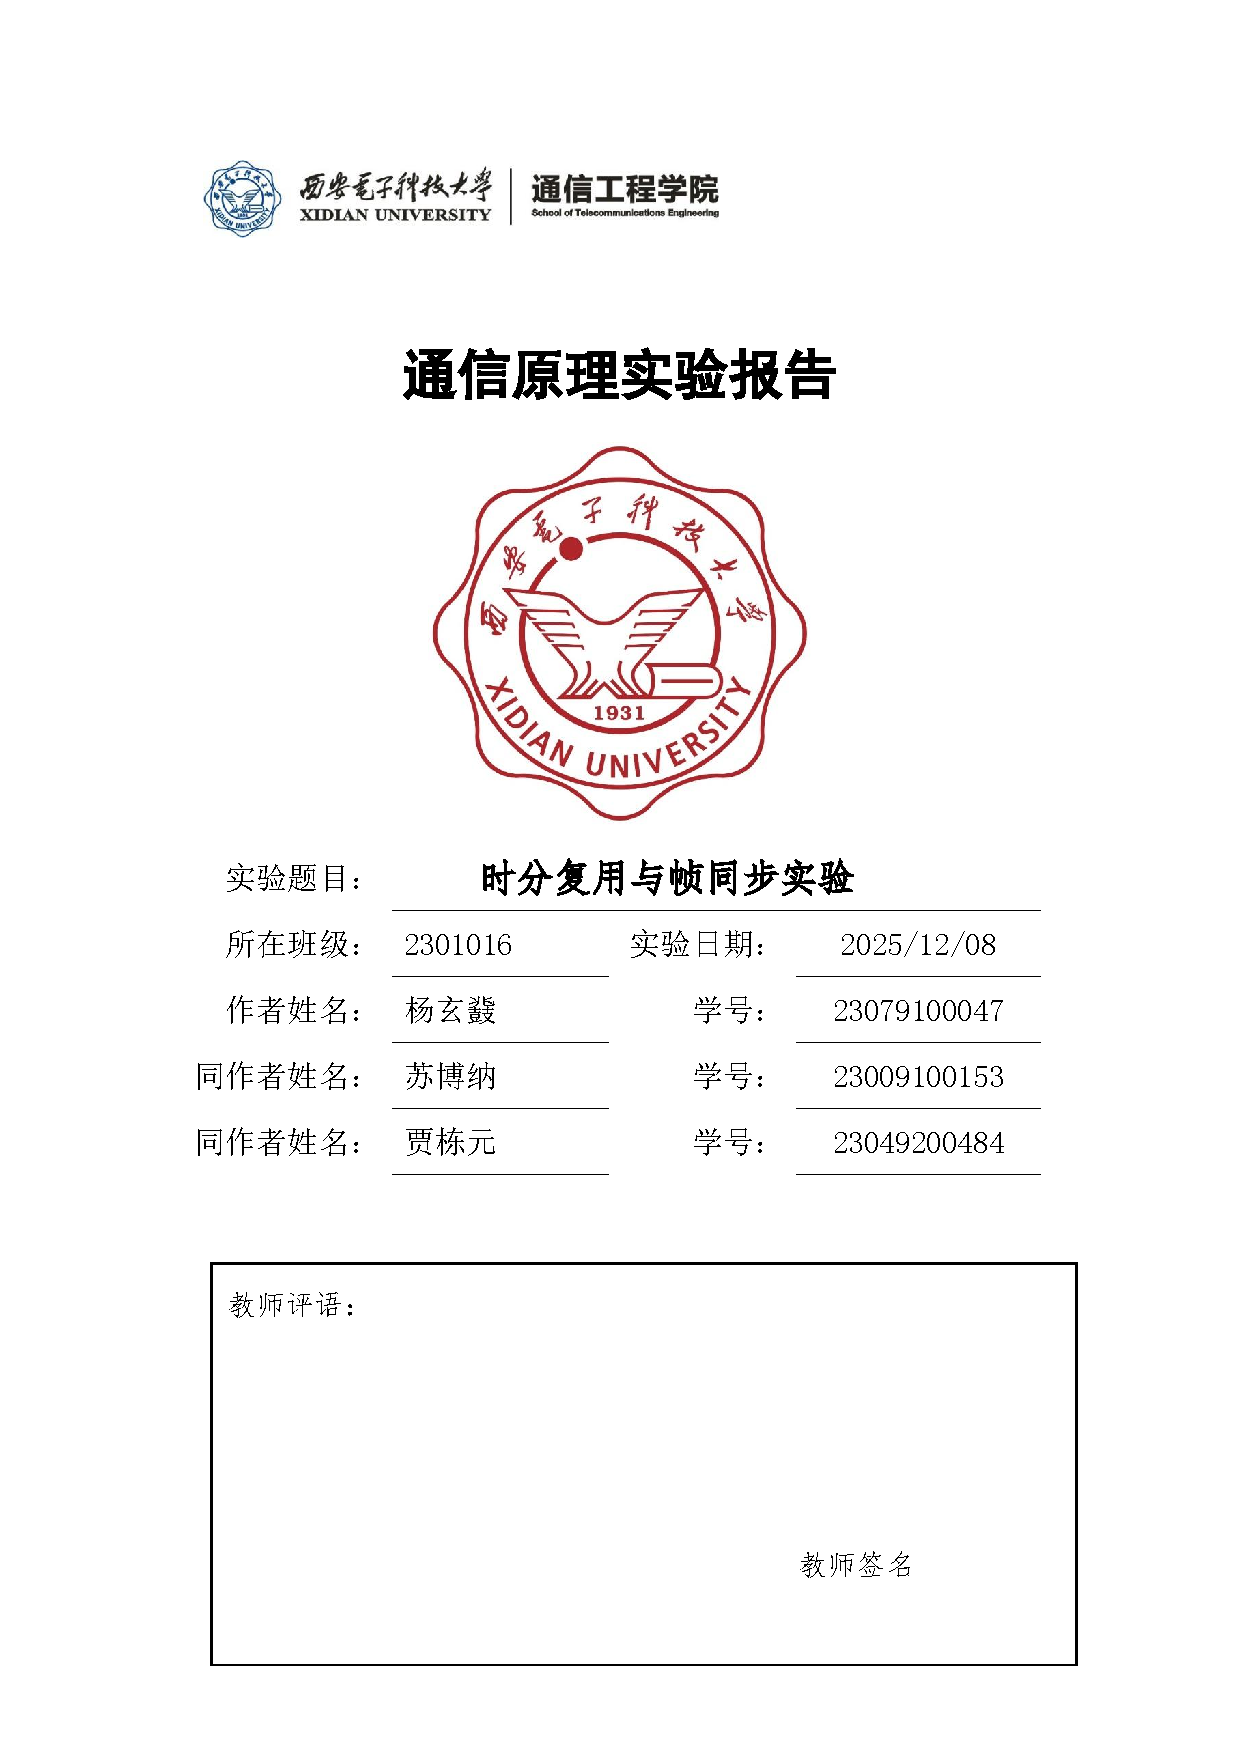
\includepdf[pages=-]{figures/实验7封面.pdf}
\end{titlepage}



% ===正文==============================


% 标题（一级居中）

\chapterinline{实验七：时分复用与帧同步实验}

\section{实验目的}
（1）掌握时分复用解复用基本原理；

（2）掌握巴克码识别原理；

（3）掌握同步保护原理；

（4）掌握假同步、漏同步、捕捉态、维持态的概念。

\section{实验器材}

西电通信与实验专业平台（半实物仿真）。

\section{实验内容}

\subsection{实验准备}

\subsubsection{获得实验权限，从浏览器进入在线实验平台；}

\subsubsection{\textbf{选择实验内容}}

使用鼠标在通信原理实验目录选择：帧同步及时分复用实验，进入到帧同步实验页面。

\subsection{发送端复接数据及帧头观测}

\subsubsection{同步帧脉冲及复接后帧头观测}

用示波器一个通道测 2TP9 帧脉冲，并将该信号作示波器同步源；另一个通道测 2P6，
观测帧头数据，分析帧头的起始位置；单击复接模块“帧头”按钮，尝试改变帧头数据，观
察帧头起始位置和帧同步的关系。可以尝试修改一些比较特殊的帧头，例如：“01111110
（0x7E）” ，“11100100（7bit 巴克码+1bit 0）”。

\textbf{实验结果：}

\begin{figure}[H]
	\centering
	\begin{subfigure}{0.45\linewidth}
		\centering
		
\includegraphics[width=\linewidth]{帧头观测（0x01111110）.png}
		\caption{帧头为 01111110 (0x7E)}
	\end{subfigure}
	\hfill
	\begin{subfigure}{0.45\linewidth}
		\centering
		
\includegraphics[width=\linewidth]{帧头观测（0x11100100）.png}
		\caption{帧头为 11100100 (7bit Barker + 1bit 0)}
	\end{subfigure}
	\caption{2TP9 帧脉冲与 2P6 复接数据中帧头的观测}
\end{figure}

\textbf{分析：}

从波形可以看到，每个帧同步脉冲（2TP9）的上升沿之后紧接着出现帧头的第一个比特。改变帧头数据仅改变帧起始处 8 bit 的模式，而不会改变帧同步脉冲的位置，说明帧同步决定帧头的起始点，
二者严格对齐并保持固定关系。

\vspace{3em}

\subsubsection{复接后 8bit 数据及各时隙数据观测}

用示波器一个通道测 2TP9 帧脉冲，并将该信号作示波器同步源；另一个通道测 2P6，
观察复用信道时隙关系及相应时隙数据，并根据实验原理所述，定位到 3 时隙 8bit 数据位
置，单击“8bit”按钮，尝试修改 8bit 编码开关，观测 2P6 的数据变化情况；

注意：结束该步骤时，要保证设置的 8-bit 数据和帧头数据不同；

\textbf{实验结果：}

\begin{figure}[H]
	\centering
	\begin{subfigure}{0.48\linewidth}
		\centering
		
\includegraphics[width=\linewidth]{8bit(0x01101101).png}
		\caption{设置 8bit 数据为 01101101 时的 2P6 波形}
	\end{subfigure}
	\hfill
	\begin{subfigure}{0.48\linewidth}
		\centering
		
\includegraphics[width=\linewidth]{8bit(0x01010101).png}
		\caption{设置 8bit 数据为 01010101 时的 2P6 波形}
	\end{subfigure}
	\caption{第 3 时隙对应的 8bit 数据在 2P6 中的变化情况}
\end{figure}

\textbf{分析：}

从波形可以看到，在帧同步脉冲之后，复用数据按固定时隙顺序依次出现，
第 3 时隙中的 8bit 数据区位置稳定可定位。当更改 8bit 编码开关时，
2P6 中第 3 时隙对应的 8bit 波形发生一致变化，而其他时隙保持不变，
说明各时隙数据在复接码流中的位置固定且相互独立。

\vspace{3em}

\subsection{帧同步提取观测及帧同步保护分析}

\subsubsection{解复用同步帧脉冲观测}

单击解复用单元“帧头”按钮，将其修改为和复用端一样的帧头数据。用示波器通道 1
观测 2TP9 帧脉冲，并作同步；另一个通道测 7TP2，观察解复用端提取的帧同步脉冲，并分
析其是否同步。

用鼠标点击复用单元和解复用单元连接开关，使其断开，观测 7TP2 是否还有帧同步脉
冲。此时输入端没有数据，无法检测到帧头，因此处于未同步状态。

尝试修改解复用“帧头”数据，将其修改为和复用端不同的帧头数据，观测 7TP2 是否
还有帧同步脉冲，思考其原因。此时，输入端虽然有数据，但是无法检测到帧头，因此处于
未同步状态.

结束该步骤时，恢复帧头同步状态，继续完成下面步骤。

\textbf{实验结果：}

\begin{figure}[H]
	\centering
	\begin{subfigure}{0.48\linewidth}
		\centering
		
\includegraphics[width=\linewidth]{解复用帧同步脉冲观测.png}
		\caption{帧头一致时的同步脉冲（7TP2 与 2TP9 对齐）}
	\end{subfigure}
	\hfill
	\begin{subfigure}{0.48\linewidth}
		\centering
		
\includegraphics[width=\linewidth]{断开开关后7TP2端同步脉冲观测.png}
		\caption{断开连接开关后，7TP2 无同步脉冲输出}
	\end{subfigure}
	
	\vspace{1em}
	
	\begin{subfigure}{0.48\linewidth}
		\centering
		
\includegraphics[width=\linewidth]{不同帧头解复用端同步脉冲观测.png}
		\caption{帧头不一致时，7TP2 无法检测同步脉冲}
	\end{subfigure}
	\caption{解复用端帧同步脉冲在不同条件下的观测结果}
\end{figure}

\textbf{分析：}

由图可见，当解复用端设置与复用端相同的帧头时，7TP2 中检测到的同步脉冲
与 2TP9 严格对齐，说明能够正确完成帧同步；当断开连接开关或设置为不同帧头时，
7TP2 不再输出同步脉冲，表明接收端无法在数据流中识别到正确帧头，处于未同步状态。

\vspace{3em}

\subsubsection{假同步测试}

假同步是指：同步系统根据其同步算法进入到了同步状态，但实际系统并没有真正同步。
设置复接发送端 8bit 数据，使其和“帧头”数据相同，用鼠标多次重复切换模块 2 和模块 7
间的开关。用示波器同时观测 2TP9 和 7TP2，观察 7TP2 是否每次都输出帧同步脉冲？7TP2
脉冲和 2TP9 脉冲是否有相差？用示波器观测原始信号 2P1 和复接-译码恢复信号 7TP7，是
否每次都相同？如不相同，分析其原因。

\textbf{实验结果：}

\begin{figure}[H]
	\centering
	\begin{subfigure}{0.48\linewidth}
		\centering
		
\includegraphics[width=\linewidth]{假同步（原始信号与恢复信号相同）.png}
		\caption{原始信号与恢复信号短暂对齐}
	\end{subfigure}
	\hfill
	\begin{subfigure}{0.48\linewidth}
		\centering
		
\includegraphics[width=\linewidth]{假同步（原始信号与恢复信号不同）.png}
		\caption{恢复信号出现相位偏移（假同步）}
	\end{subfigure}
	\caption{假同步情况下原始信号与解复用信号的对齐与错位现象}
\end{figure}

\textbf{分析：}

当复接端设置的 8bit 数据与帧头完全相同时，数据流中会出现多个与真实帧头一致的模式，
解复用端可能将错误位置误判为帧头，从而进入假同步状态。此时 7TP2 的同步脉冲虽然仍周期性输出，但帧起始点并不正确，因此恢复信号的时隙划分也随之偏移。

用示波器比较原始输入信号 2P1 和恢复信号 7TP7 可以看到，二者并不是每次都完全一致。
当解复用端误将某个错误位置当作帧起始点时，7TP7 的信号会相对于 2P1 产生错位。其根本原因是：系统虽然“认为已经同步”，但实际帧头位置错误，
导致后续时隙全部被分配到错误位置。

\vspace{3em}

\subsubsection{后方保护测量（捕捉态）}

帧同步提取中，增加了后方保护，后方保护是为了防止伪同步的不利影响。后方保护是
这样防止伪同步的不利影响的：在捕捉帧同步码的过程中，只有在连续捕捉到 n（n 为后方
保护计数）次帧同步码后，才能认为系统已真正进入到了同步状态。后方保护的前提是在后
方保护之前，系统处于捕捉状态。

将示波器分别观测：发送端帧同步脉冲 2TP9，接收端检
测的帧同步脉冲 7TP2。单击“前向保护”按钮，弹出 16bit
拨码开关。将 16bit 设置为全“1”，则连续 16 帧数据帧头全
部加错，观测此时 7TP2 是否有帧脉冲输出？逐渐增加正确
帧头个数(将拨码开关设置为 0)，如：1bit、2bit、3bit、4bit…
（连续的 n-bit），观测 7TP2 是否有帧头输出，根据结论分析
后方保护计数 n 的个数；

后方保护时间是指：从捕捉到第一个同步码到系统进入同步状态这段时间称为后方保护
时间，可表示为 Td；尝试分析后方保护时间 Td.

\textbf{实验结果：}

\begin{figure}[H]
	\centering
	\begin{subfigure}{0.48\linewidth}
		\centering
		
\includegraphics[width=\linewidth]{后方保护（14bit0）.png}
		\caption{仅少量帧头错误时仍可输出同步脉冲}
	\end{subfigure}
	\hfill
	\begin{subfigure}{0.48\linewidth}
		\centering
		
\includegraphics[width=\linewidth]{后方保护（3bit0）.png}
		\caption{错误帧头变多后无法输出同步脉冲}
	\end{subfigure}
	\caption{部分帧头错误时 7TP2 同步脉冲的变化情况}
\end{figure}

\begin{figure}[H]
	\centering
	
\includegraphics[width=0.55\linewidth]{后方保护（全1时、无帧脉冲输出）.png}
	\caption{帧头全部错误（设置为全1）时，7TP2 完全无同步脉冲输出}
\end{figure}

\textbf{分析：}

从图中可以看出，当只有少量帧头被破坏时，7TP2 仍能输出帧同步脉冲；而当错误帧头
数量增多时，7TP2 不再输出同步脉冲，说明接收端在捕捉态只有在连续捕获到足够多的
正确帧头后，才会判定进入同步状态。由示波器波形统计可知，需要连续捕获 $n$ 帧正确
帧头后 7TP2 才开始稳定输出同步脉冲，因此本系统的后方保护计数为 $3$ 帧。

由 2TP9 相邻帧同步脉冲之间的时间间隔可测得帧周期为 $T_f$（本实验中约为
$T_f \approx 125~\mu\text{s}$），则从捕捉到第一个正确帧头到系统真正进入同步状态
所经历的时间为
\[
T_d = n T_f =375~\mu\text{s},
\]
这段时间即为后方保护时间。可见，后方保护时间与所要求的连续正确帧头个数 $n$ 成正比，
$T_d$ 越大，系统进入同步状态越“谨慎”，对偶然出现的假同步码更不敏感，但同步建立
的速度也会相应变慢。



\subsubsection{前向保护测试（维持态）}

系统在进入同步状态后设置了前方保护，前方保护是为了防止假失步的不利影响。前方
保护是这样防止假失步的不利影响的：当同步系统检测不到同步码时，并不立即进入捕捉态，
而是当连续 m 次（m 称为前方保护计数）检测不到同步码后，才判为系统真正失步，然后
进入捕捉状态，重新开始捕捉同步码。

将示波器分别观测：发送端帧同步脉冲 2TP9，接收端检测的帧同步脉冲 7TP2。单击“前
向保护”按钮，弹出 16bit 拨码开关。将 16bit 设置为全“0”，则连续 16 帧数据帧头均未加
错，观测此时 7TP2 帧脉冲是否正确？逐渐增加错误帧头个数(将拨码开关设置为 1)，如：
1bit、2bit、3bit、4bit…（连续的 n-bit），观测 7TP2 帧同步检测信息是否有丢失，用示波器
观测 2P1 和 7TP7，是否相同？。根据结论分析前向保护计数 n 的个数；

尝试观测当开关位置为“0001000100010001”、“0010010110010011”时，帧同步提取情
况和解复用-译码信号恢复情况；

前方保护时间是指：从第一个帧同步码丢失起到帧同步系统进入捕捉状态为止的这段时
间称为前方保护时间，可表示为：Ts；尝试分析前向保护时间 Ts.


\textbf{实验结果：}

\begin{figure}[H]
	\centering
	\begin{subfigure}{0.45\linewidth}
		\centering
		
\includegraphics[width=\linewidth]{前向保护（2bit1时有同步检测信息丢失）.png}
		\caption{少量连续错误帧头（如 2bit 错误）时同步情况}
	\end{subfigure}
	\hfill
	\begin{subfigure}{0.45\linewidth}
		\centering
		
\includegraphics[width=\linewidth]{前向保护（0001000100010001同步和译码情况）.png}
		\caption{间隔性错误模式 ``0001000100010001'' 的同步情况}
	\end{subfigure}
	
	\vspace{1em}
	
	\begin{subfigure}{0.45\linewidth}
		\centering
		
\includegraphics[width=\linewidth]{前向保护（0010010010010011同步和译码情况）.png}
		\caption{间隔性错误模式 ``0010010110010011'' 的同步情况}
	\end{subfigure}
	\hfill
	\begin{subfigure}{0.45\linewidth}
		\centering
		
\includegraphics[width=\linewidth]{前向保护（全0时）.png}
		\caption{16bit 全为 0（无错误帧头）时同步情况}
	\end{subfigure}
	
	\caption{前向保护条件下不同帧头错误模式对应的同步脉冲与译码信号观测}
\end{figure}

\textbf{分析：}

少量连续错误帧头（如仅 1--2bit 连续为 1）时，7TP2 的同步脉冲偶尔会出现丢失，
但在下一帧重新检测到正确帧头后即可恢复。此时原始信号 2P1 与恢复信号 7TP7 基本一致，
系统仍然保持同步状态，前向保护对短暂、轻微错误具有容忍性。

当错误采用 ``0001000100010001''、``0010010110010011'' 等间隔分布模式时，
尽管部分帧头错误，但因为错误不连续、不会形成连续 $m$ 帧的同步检测失败，
系统始终能够稳定输出同步脉冲，2P1 与 7TP7 波形一致，说明前向保护仅对
“连续错误帧头”敏感，而对间隔性错误不敏感。

当 16bit 全为 0（等于完全正确帧头）时，系统能持续成功检测同步码，7TP2 均匀输出同步脉冲，
恢复信号与原信号完全一致，说明系统在无错误条件下可保持稳定同步。

随着错误比特数增加，当错误帧头连续达到一定数量时，7TP2 的同步脉冲完全消失，
系统进入失步状态。由实验可估计系统的前向保护计数约为
\[
m = 13
\]

前向保护时间定义为：从检测到第一个同步码丢失开始，到系统判定失步为止所需的时间，
记为 $T_s$。设帧周期为 $T_f$，则有
\[
T_s = m T_f.
\]
前向保护时间越长，系统越能抵抗偶发错误，但进入失步的反应也越慢。本实验中以
$T_f \approx 125~\mu\text{s}$ 计，则
\[
T_s \approx 125 m ~\mu\text{s}.
\]

\subsubsection{同步状态下音频观测}

将系统设置到同步状态，完成下列内容：用示波器观测 7TP7 和 7TP8，比较输出信号和 2P1 输入信号是否一致；分析 2P1 和 7TP8相位不一致（延时）的主要原因？

\textbf{实验结果：}

\begin{figure}[H]
	\centering
	
\includegraphics[width=0.5\linewidth]{同步时相位不一致.png}
	\caption{同步状态下输入信号 2P1 与 PCM 恢复信号 7TP8 的波形比较}
\end{figure}

\textbf{分析：}

对比 2P1 与 7TP8 可以发现，两者存在固定的相位滞后（时间延时）。

该相位（延时）主要由系统内部的数字处理链路引起：输入模拟信号需经 A/D 采样、
PCM 编码或 CVSD 编码、时分复用成帧、在接收端完成帧同步与解复用、再经译码和 D/A
重构以及低通滤波等多个环节，每个环节都会引入若干个采样周期或若干帧周期的群时延。
这些延时累加后表现为 7TP8 相对于 2P1 的整体滞后，因此在同步状态下虽然波形一致，
但相位（时间位置）并不完全重合。

\section{实验报告要求}

\subsection{帧同步基本原理}

在时分复用（TDM）系统中，多路语音或数据以固定的帧结构复接到一条高速数字链路上。
每一帧均由帧头（同步码）与若干时隙构成。为了保证接收端能够正确识别各路信号在
帧中的位置，必须在接收端实现帧同步。

帧同步的核心任务是在接收端码流中准确定位每一帧的起始位置。系统通常采用预先设计的
帧同步码作为帧头，该码型应具有良好的自相关特性，使其在随机数据中出现的概率极低，
从而便于接收端通过相关检测方法识别。接收端通过滑动相关或模式匹配的方法寻找帧头，
当检测到与同步码高度匹配的序列时，即认为找到了一帧的开始。

由于噪声、码间干扰或数据模式偶合等因素，码流中可能偶尔出现与帧同步码相似的序列，
导致接收端误判同步位置，因此需要引入保护机制。为了避免误同步，系统设置了“后方保护”
（捕捉态保护）：只有在连续检测到 $n$ 次有效同步码后，系统才确认同步成立，进入同步状态。
这样可以有效避免因偶然相关峰值造成的假同步。

进入同步状态后，系统仍需防止因短时错误导致误失步。为此，引入“前向保护”（维持态保护）：
如果某一帧未检测到同步码，接收端并不立即判定失步，而是要求连续 $m$ 次检测不到同步码
才认为真正失步，并重新进入捕捉阶段。该机制可有效抑制偶发错误带来的假失步。

通过这些机制，系统能够在复杂信道环境下实现稳定可靠的帧同步。


\subsection{完成实验步骤，并记录相关波形及实验结论；}

相关波形及实验结论见第三节。

\subsection{画出实验中帧同步的状态机；}

\begin{figure}[H]
	\centering
	
\includegraphics[width=0.5\linewidth]{帧同步状态机.png}
	\caption{帧同步状态机}
\end{figure}

\subsection{帧同步过程及前后向保护作用}

帧同步过程可分为三个阶段：捕捉、同步维持、失步重捕捉。

在捕捉阶段，接收端利用相关检测方法在码流中寻找帧头模式。由于噪声和数据随机性，
偶然出现的假帧头可能导致错误同步，因此系统设置了后方保护机制：只有当连续检测到
$n$ 个正确帧头时，才认为真正同步。该机制有效避免了因偶然相关峰值造成的假同步。

在同步维持阶段，系统已进入稳定同步状态。为了防止因瞬时干扰或单帧错误导致误判失步，
系统加入前向保护机制：如果某一帧未检测到帧头，不立即失步，而是开始前向保护计数。
只有当连续 $m$ 帧均未检测到有效帧头时，系统才判定真正失步，重新进入捕捉阶段。
该机制有效抑制了“假失步”。

实验中观察到：轻微或间隔性错误不会导致失步，而连续大量错误帧头才能触发失步，
验证了前向保护的可靠性；同时，只有在连续捕获到若干个有效帧头后系统才会进入同步，
也验证了后方保护的作用。



\section{实验思考题}

\subsection{如果希望开关设置为“0111011101110111”时系统仍能同步，则状态机应怎么修改？}

序列“0111011101110111”中包含多个与帧头部分相似的模式，如果采用严格的
“连续 $n$ 帧均检测到完整帧头”作为同步条件，则系统可能无法从该序列中稳定提取
有效同步信息。若希望在此类码型下系统仍能同步，需要对帧同步状态机做如下修改：

\begin{enumerate}
	\item 将同步判决条件由“连续 $n$ 次完整匹配”调整为
	“相关值超过阈值 $T$ 的累计次数超过一定数量”，即采用“加权累计判决”；
	\item 或将状态机修改为“在固定窗口内检测到若干次有效相关峰值”即可进入同步，
	而不要求连续出现；
	\item 另一种方法是将同步码检测由“硬判决匹配”改为“软判决相关匹配”，允许部分比特错误；
	\item 也可适当降低同步阈值，使得序列中“近似帧头”也能被视为有效同步信号。
\end{enumerate}

修改后的状态机可表示为：

\[
\text{若在 } W \text{ 帧窗口内检测到 } K \text{ 次有效相关峰值，则进入同步态。}
\]

其中 \( W \) 和 \( K \) 可根据同步可靠性需求选取。  
这样，即便帧头受到扰动或与“0111011101110111”类似，也能够成功同步。

\subsection{查阅相关资料，说明什么是帧同步后向保护？实验原理部分状态机中有没有后向保护功能？保护几帧？}

帧同步的后向保护是指：当接收端在某一帧检测不到同步码时，
并不立即判定同步失败，而是继续观察后一帧或数帧的检测结果。当随后检测到正确帧头
时，即“向后回溯”认为当前同步仍然有效，从而避免因单帧错误导致误失步。

结合实验指导书和本次实验状态机可知：  
实验系统 \textbf{没有显式实现帧同步后向保护}，而是通过“前向保护”完成类似功能，
即要求连续 $m$ 帧检测不到同步码才真正失步。

从实验结果可知：系统对连续 \( 13 \) 帧同步码缺失具有容忍能力；  
但若缺失帧数不足 \( m \)，系统直接保持同步，并不会回溯修正同步位置。



\end{document}